\documentclass[12pt]{article}

\usepackage[top=1in,bottom=1in,left=1in,right=1in]{geometry}
\usepackage{amsmath,amssymb,mathtools}
\usepackage{xcolor}
\usepackage{graphicx}
\usepackage{hyperref}
\usepackage{enumitem}

\hypersetup{
    pdfauthor={},
    pdftitle={MATH 1075 - Lesson 6.1 Recitation}
}

\begin{document}

\vspace*{0.5in}

\begin{center}
    {\LARGE MATH 1075 - Section 8.3 - 8.4 Worksheet}

    \vspace{2em}

    {\large 10/08/2026}
\end{center}
\section{Linear, Constant, and Quadratic Function}
Identify if the function is linear, constant, quadratic, or neither
\vspace{1.5em}

1. $f(x)=x^{2}+5x+2$

\vspace{3.5em}

2. $f(x)=\frac{1}{2} $

\vspace{3.5em}

3. $f(x)=\frac{3}{2}x-\frac{1}{4} $

\vspace{3.5em}

4. $f(x)=\left\vert \frac{2}{3}x+6 \right\vert$

\vspace{3.5em}

5. $f(x)=\sqrt{5}$

\newpage
\section{$x$-intercept, $y$-intercept}
Find the $x$-intercept(s) and $y$-intercept of the function and graph the function.\\
1. $f(x)=2x+9$ 
\begin{figure}[htbp]
    \centering
    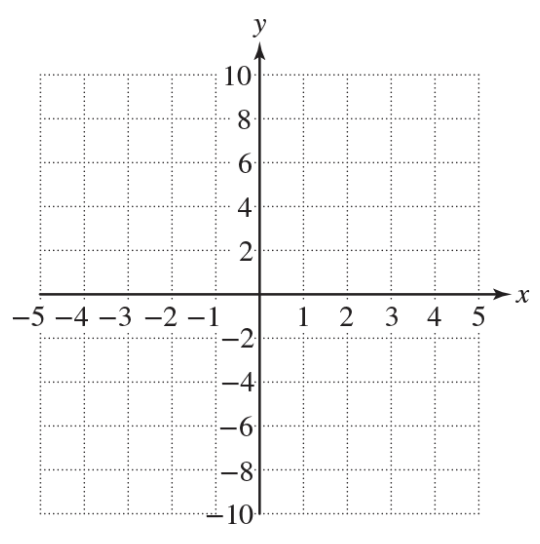
\includegraphics[width=0.31\linewidth]{Screenshot 2026-10-07 at 1.06.38 PM.png} 
\end{figure}\\
2. $f(x)=18$
\begin{figure}[htbp]
    \centering
    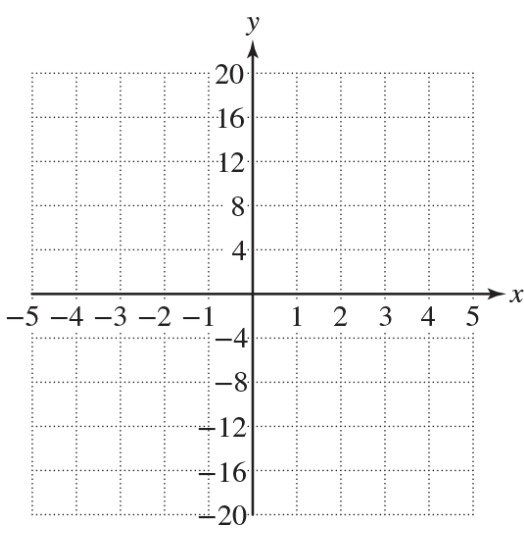
\includegraphics[width=0.31\linewidth]{Screenshot 2026-10-07 at 1.10.07 PM.png} 
\end{figure}\\
3. $f(x)=x^{2}-1$
\begin{figure}[htbp]
    \centering
    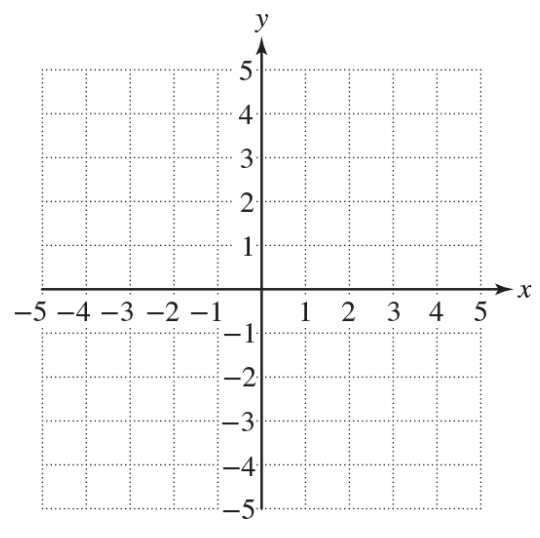
\includegraphics[width=0.31\linewidth]{Screenshot 2026-10-07 at 1.10.36 PM.png} 
\end{figure}

\newpage 
\section{Algebra and Composition of Functions}
Given $f(x)=x+4$, $g(x)=2x^{2}+4x$, $h(x)=x^{2}+1$ find:
\vspace{1.5em}

1. $(f+g)(x)$

\vspace{3.5em}

2. $(g-f)(x)$

\vspace{3.5em}

3. $(f\cdot h)(x)$

\vspace{3.5em}

4. $\left(\frac{f}{h} \right)(x)$

\vspace{3.5em}

5. $(f+g)(2)$

\vspace{3.5em}

6. $(g-f)(1)$

\vspace{3.5em}

7. $(f\cdot h)(0)$

\vspace{3.5em}

8. $\left(\frac{f}{h} \right)(3)$

\newpage

\noindent Given $f(x)=\sqrt{x+6}$ and $g(x)=x^{2}+1,$ find:

\vspace{1.5em}

1. $(f\circ g)(x)$

\vspace{3.5em}

2. $(g\circ f)(x)$

\vspace{3.5em}

3. $(f\circ g)(3)$

\vspace{3.5em}

4. $(g\circ f)(3)$

\vspace{4.5em}
Given a graph find:
\begin{figure}[htbp]
    \centering
    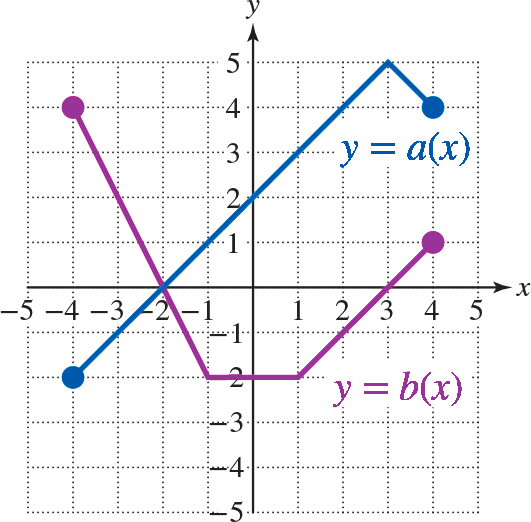
\includegraphics[width=0.4\linewidth]{mil73537_sec_pra_ex0804067.png} 
\end{figure}

1. $a(-1)$

\vspace{1.5em}

2. $(a+b)(1)$ 

\vspace{1.5em} 

3. $(a\circ b)(-2)$ 

\vspace{1.5em} 

4. $(b\circ a)(0)$
\end{document}
